\section{Ablation Studies}

In ablation studies, we investigated the individual importance of the following modules: Curriculum Strategy, input and reward normalization, actuator-width information, and the shaped reward. All ablation study experiments were carried with the SAC algorithm with depth perception and one million experience replay buffer size. Every ablation training took place in the full environment floor scene. We shared the results of ablation studies in the same table as the SAC full environment [REF to table].

\begin{figure}[htbp]
    \begin{subfigure}{0.49\textwidth}
        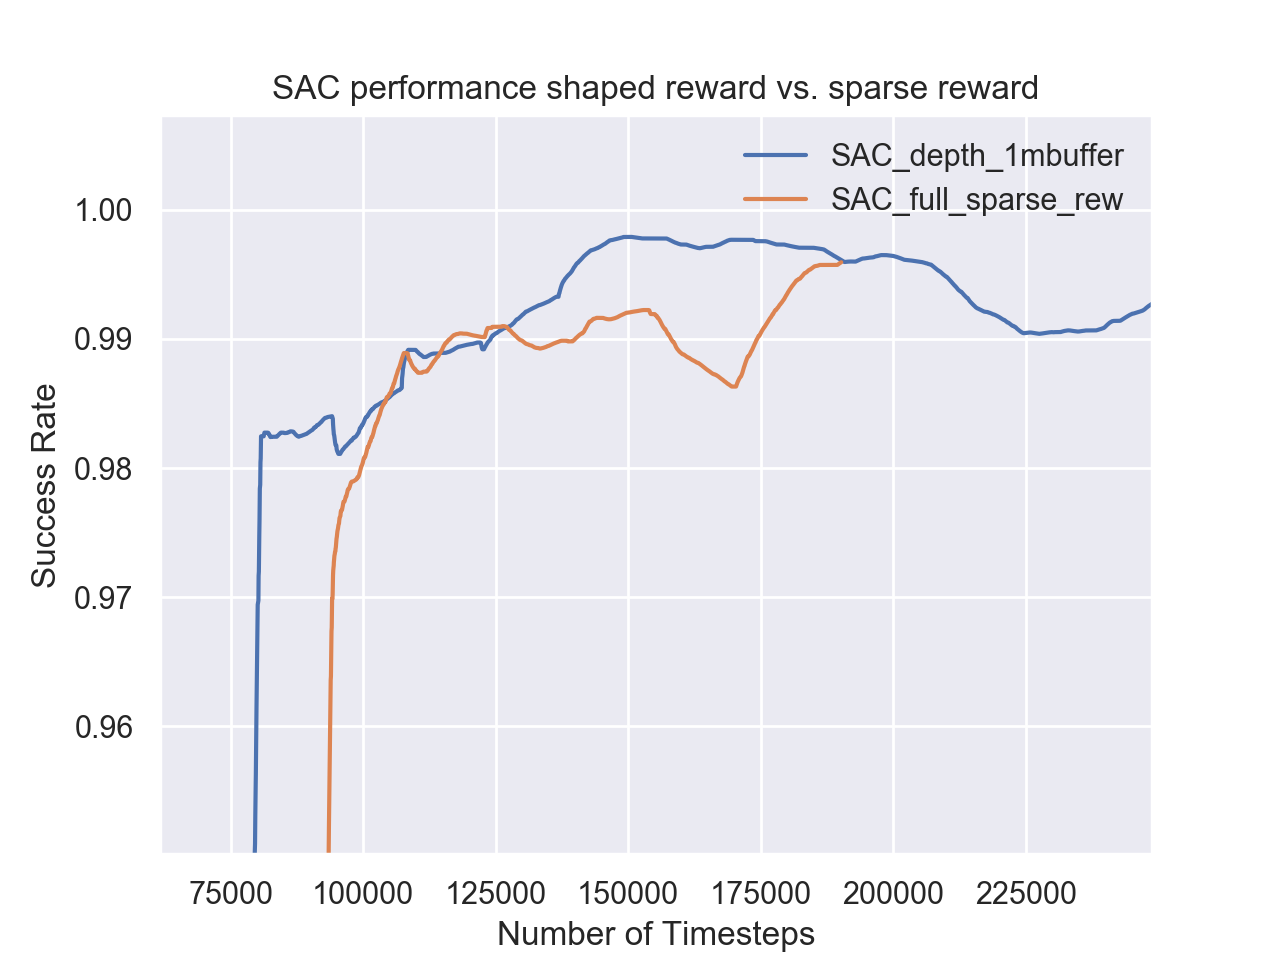
\includegraphics[width=\linewidth]{figures/ablation/SAC_performance_shaped_reward_vs_sparse_reward}
        \caption{Table Scene} \label{fig:table}
    \end{subfigure}%
    \hspace*{\fill}   % maximize separation between the subfigures
    \begin{subfigure}{0.49\textwidth}
        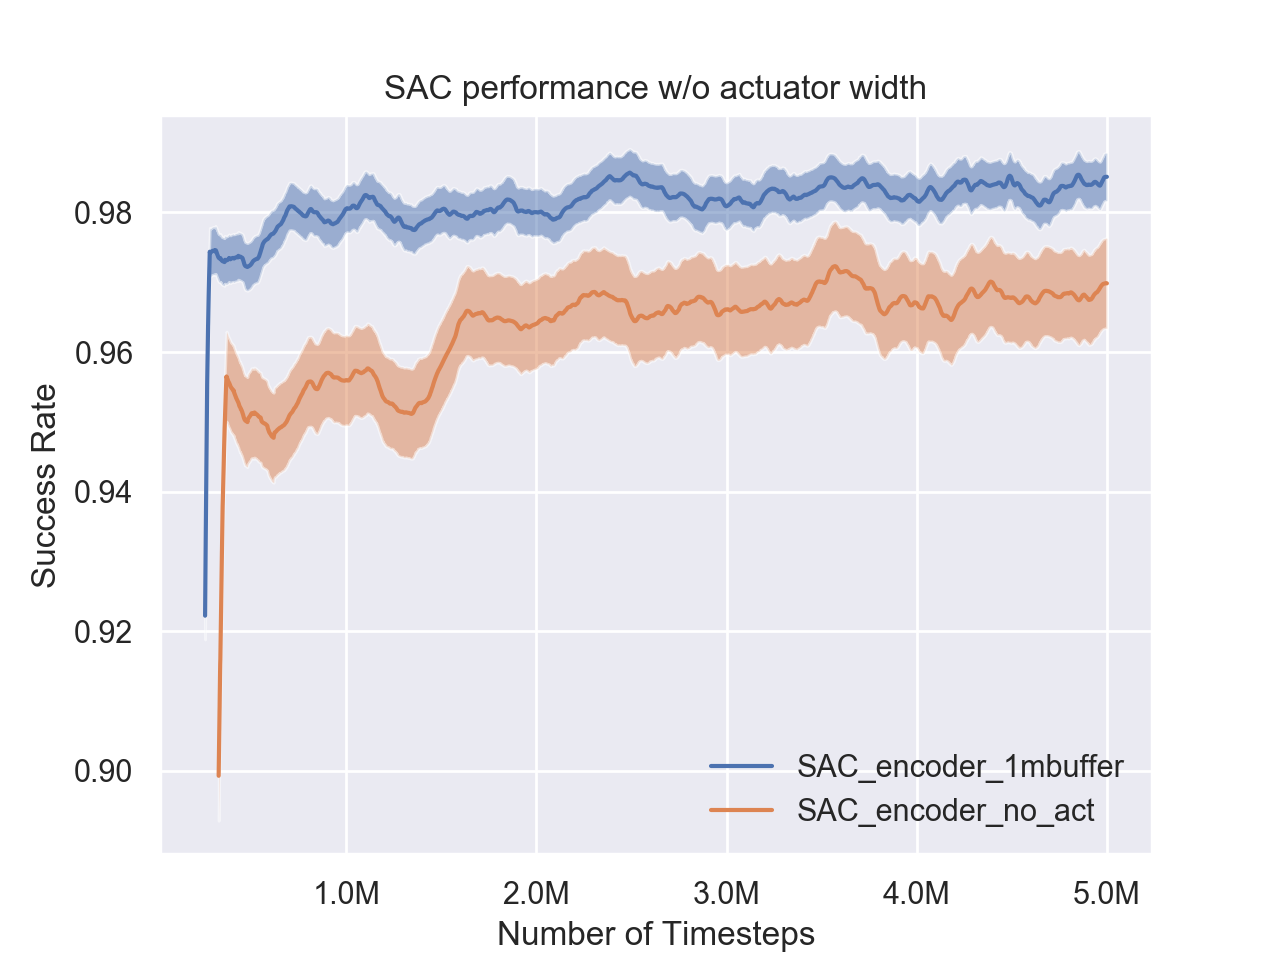
\includegraphics[width=\linewidth]{figures/ablation/SAC_performance_wo_actuator_width}
        \caption{Floor Scene} \label{fig:floor}
    \end{subfigure}%
    \hspace*{\fill}   % maximize separation between the subfigures


\caption{ Table and floor scenes \label{fig:scenes}}
\end{figure}

